\chapter{User manual}
\label{chap:manual}

\par This chapter is a guide, going through all the steps for using the application

\section{Starting the application}
\label{sec:manualsec1}

\section{Starting the recording}
\label{sec:manualsec2}

\begin{figure}
    \centering
    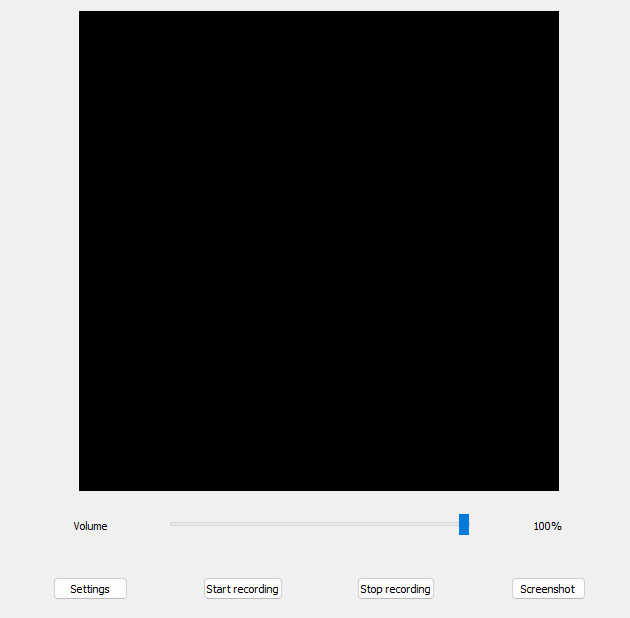
\includegraphics[width=0.5\linewidth]{figures/MainPage.png}
    \caption{How the Main page looks right after starting the application}
    \label{fig:MainPageLooks}
\end{figure}

\par When being on the Main page, seen at image\ref{fig:MainPageLooks}, starting the recording is as simple as pressing the "Start recording" button. After 1 or 2 seconds, the recording start, which can be seen when the black square changes to the live camera feed, like in image\ref{fig:MainPageRecordingLooks}.

\begin{figure}
    \centering
    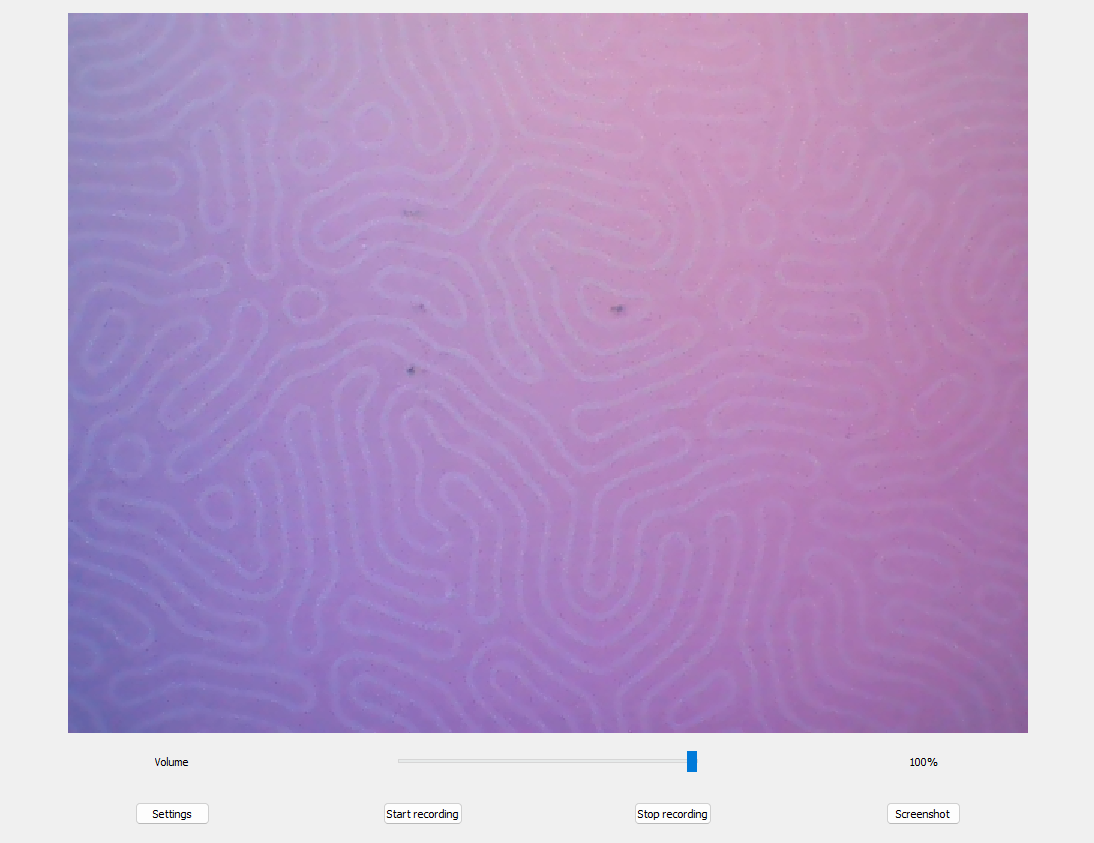
\includegraphics[width=0.5\linewidth]{figures/MainPageRecording.png}
    \caption{How the Main page looks when recording a video}
    \label{fig:MainPageRecordingLooks}
\end{figure}

\par While the video is being recorded, the visual part is saved in real-time to the folder selected in the settings, named as TempRecording, as seen in image\ref{fig:TempRecordingLooks}. This file is not the whole video, the audio part is merged with the visual when the recording stops, and opening it until it is finished is not advised, since the behaviour of the application in that case is unknown.

\begin{figure}
    \centering
    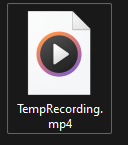
\includegraphics[width=0.15\linewidth]{figures/TempRecording.png}
    \caption{The visual file in the video folder}
    \label{fig:TempRecordingLooks}
\end{figure}